\chapter{Theoretical foundation}
\label{ch:theory}

% The problem examined in this thesis is assisted lane keeping with shared control by a potentially distracted human driver and an agent. The agent acts as an \gls{adas} to assis the driver in keeping the car centered in its lane. The driver's attentiveness and the exact position of the car are unknown to the agent. 

% TODO: What problem? Quick recap
In this chapter, the basic theoretical concepts which serve as a foundation to formally model the problem and to solve it are presented. The task involves sequential decision making, where every prior decision influences the following ones. Section \ref{sec:mdp} shows how sequential decision making tasks can be formulated using \Glspl{mdp}. However, since the agent only observes partial information, uncertainty about the driver's attentiveness and the car's road position is involved. Section \ref{sec:pomdp} introduces the \Gls{pomdp}, which is an extension of an MDP, accounting for partial observability of information. It is well suited to model the uncertainty involved in the problem. Solving POMDP is a difficult task. Section \ref{sec:challenges} discusses the key challenges involved in solving POMDP. Many solution approaches have been proposed. In section \ref{sec:solvers} an overview over proposed solvers is provided.

\section{Sequential decision making}
\label{sec:mdp}

Lane keeping of a car is a sequential decision making task. Every steering action that is performed directly influences the choice of the best succeeding steering actions. \Glspl{mdp} are well suited and widely used to model sequential decision making tasks. An \gls{mdp} is a discrete time framework for a decision maker, the agent, to interact with an environment. At every time step, the environment is in a certain state, fully observable by the agent. The agent interacts with the environment by performing an action that determines the next state of the environment. The underlying assumption, the Markov property, is that the next state of the environment only depends on its current state and the agent's action. The transition to a succeeding state after an action has been performed does not need to be deterministic but can be probabilistic, accounting for randomness in the environment. After performing an action, the agent receives a numerical reward (also called return). The agent's goal is to maximize the cumulative reward it receives over time. An action that leads to a high immediate return is not optimal if another action leads to a higher cumulative reward in the long run. Thus, the agent needs to find an optimal policy that decides the best action to take in every state. In case the state transition probabilities are known to the agent, the optimal policy can be found using model-based techniques such as value or policy iteration. If the transition model is unknown, model-free reinforcement learning can be applied to learn an optimal policy. % TODO: Add source

\begin{figure}[htbp]
    \centering
    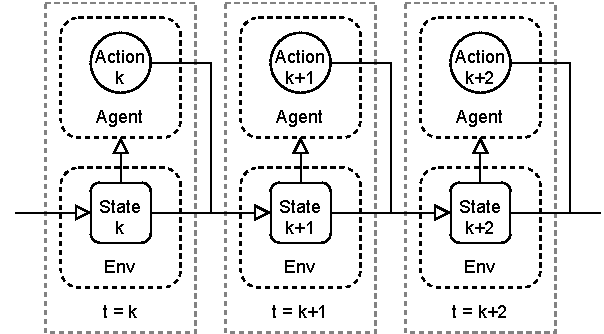
\includegraphics[width=0.75\textwidth]{figures/MDP.pdf}
    \caption{\acrfull{mdp}}
\end{figure}

Assisting a human driver in the lane keeping task is essentially a sequential decision making task as well. However, the agent that is assisting the human driver does not know about the driver's internal psychological state, and therefore her attention. A distracted driver may steer poorly and needs assistance. But how can the agent tell whether the driver is distracted? Reading the driver's mind is not feasible and even if it were, it would be too invasive for this task. Instead, the agent needs to estimate the driver's internal state in order to act adequately. A \Gls{pomdp} is a generalization of an MDP that allows to plan under uncertainty. Even without observing the full state of the agent's environment, of which the driver is part of, a POMDP allows the agent to estimate the environment's true state using the partial information it observes. A POMDP serves as the foundation of this thesis. The lane keeping assistance problem this thesis aims to solve can be defined as a POMDP. First, a formal definition is needed.

\section{Partially observable Markov decision process (POMDP)}
\label{sec:pomdp}
% See POMDP Model from (POMDP algorithm) Online Planning Algorithms for POMDPs

The POMDP generalizes the MDP for planning under uncertainty. The environment's true state is unknown to the agent. It has to rely on observations with partial information about the environment's true state to choose its actions. \cite{pomdp-definition} define a POMDP as a tuple $(S, A, T, R, O, Z)$, where:
\begin{itemize}
    \item $S$ is the set of all possible states $s \in S$ of the environment. A state describes the environment at a time point. It must not be an all-encompassing description but must include all relevant information to make decisions. The state is hidden from the agent. This is the main difference to an MDP.
    \item $A$ is the set of all possible actions $a \in A$ the agent can perform in the environment.
    \item $T : S \times A \times S \rightarrow [0,1]$ defines the conditional state transition probabilities. $T(s,a,s') = Pr(s' | s, a)$ constitutes the probability of transitioning to state $s'$ after performing action $a$ in state $s$.
    \item $R : S \times A \rightarrow \R$ is the reward function providing the agent with a reward of $R(s,a)$ after performing action $a$ in state $s$.
    \item $O$ is the set of all possible observations $o \in O$. Observations are the agent's source of information about the environment, enabling the agent to estimate the environment's state.
    \item $Z : S \times A \times O \rightarrow [0,1]$ defines the conditional observation probabilities. $Z(s', a, o) = Pr(o | s', a)$ represents the probability of receiving observation $o$ at state $s'$ after performing action $a$ in the previous state. 
\end{itemize}

At any time, the environment is in some state $s$. Unlike in the case of an MDP, the agent cannot directly observe the environment's state. Instead, the agent receives an observation $o$ that provides partial information about the current state. The agent uses the observations it perceives over time to estimate the true state of the environment in order to choose adequate actions. At any time step $t$, it has to take into account the complete history $h_t$ of actions and observations until $t$:

\begin{equation}
    h_t = \{a_0,o_1,...,o_{t-1},a_{t-1},o_t\}
\end{equation}

Keeping a collection of all past observations and actions is very memory expensive. A less memory demanding alternative is to only keep a probability distribution over the states at every step, called a belief $b$. $b(s,h)$ denotes the probability of being in state $s$ given history $h$. 

\begin{equation}
    b_t(s,h) = Pr(s_t = s|h_t = h)
\end{equation}

The belief is a sufficient statistic for the agent to form a decision about its next action \parencite{pomdp-belief}. Thus, only the belief needs to be kept and can be recursively updated whenever an action is performed and a new observation arises. The agent starts with an initial belief $b_0$ about the initial state of the environment. At every subsequent time step, the new belief $b'$ can be recursively calculated based on the previous belief $b$, the last action $a$ and the current observation $o$. The previous belief can then be discarded as the history it represents is no longer up-to-date. For an exact update of the belief one can apply the Bayes theorem:

\begin{equation}
    \label{eq:bayes_update}
    \begin{split}
        b'(s') & = Pr(s' | o, a , b) \\
               & = \frac{Pr(o | s', a, b)Pr(s' | a,b)}{Pr(o| a, b)} \\
               & = \frac{Pr(o | s', a)\sum_{s \in S}Pr(s' | a, b, s)Pr(s| a, b)}{Pr(o| a, b)} \\
               & = \frac{Z(s', a, o)\sum_{s \in S}T(s, a, b)b(s)}{Pr(o | a, b)}
    \end{split}
\end{equation}

The agent chooses its actions based on its belief according to its policy $\pi$. The agent's policy defines the action to choose at any given belief state. It describes the strategy for every possible situation the agent can encounter. Solving a \gls{pomdp} consists in finding an optimal policy $\pi^*$ that maximizes the the cumulative reward obtained over some time horizon $N$ starting from initial belief $b_0$ using a discount factor $0 \leq \lambda \leq 1$:

\begin{equation}
    \pi^* = argmax_{\pi}~E\left[ \sum_{t=0}^{N} \sum_{s \in S}b_t(s) \sum_{a \in A} \lambda^t R(s,a) \pi(b_t,a) | b_0\right]
\end{equation}

% Value function
The return that is gained by following a policy $\pi$ from a certain belief $b$ can be obtained with the value function $V^\pi(b)$:

\begin{equation}
    V^\pi(b) = \sum_{a \in A} \pi(b,a) \left[ \sum_{s \in S} b(s) R(s,a) + \lambda \sum_{o \in O} Pr(o | b, a) V^\pi(b')\right]
\end{equation}

The optimal policy $\pi^*$ maximizes $V^\pi(b_0)$. For any POMDP there exists at least one optimal policy.

\section{Key challenges}
\label{sec:challenges}

\subsection{Curse of dimensionality and curse of history}
\label{sec:curses}

Computing an optimal policy for a POMDP is challenging for two distinct but interdependent reasons \parencite{pomdp_curses}. On the one hand, there is the so-called curse of history: Finding an optimal policy is like searching through the space of possible action-observation histories. The number of distinct histories grows exponentially with the size of the time horizon. Therefore, planning further into the future increases the computation complexity exponentially. While finding an optimal policy can be relatively easy for short histories, it becomes computationally infeasible for larger time horizons. On the other hand, there is the curse of dimensionality: The belief space is ($|S|$-dimensional. Therefore, the size of the belief space, representing the number of states in a POMDP, grows exponentially with $|S|$.

The task of finding an optimal policy for a finite horizon POMDP is PSPACE-complete \parencite{pomdp_complex}. Solving POMDP to optimality is computationally infeasible with a large state space or time horizon. For this reason, approximate algorithms are often applied. 

\subsection{Unknown transition and observation probabilities}
\label{sec:gen_model_intro}
For many problems, it is difficult or impossible to know the probability distributions $T$ or $Z$ explicitly. This is also the case for the shared control lane keeping scenario assessed in this thesis. Neither the transition probabilities, nor the observation probabilities are known a priori. The belief update method using Bayes' theorem presented in Equation \ref{eq:bayes_update} is not computable without knowing the probabily distributions explicitly. However, exact updates are too complex for problems with a large state space in any case \parencite{pomcp}. Some solution approaches circumvent the problem of unknown transition and observation probability distributions by only requiring a generative model that can sample state and observation transitions. A generative model can stochastically generate a successor state, reward, and observation, given the current state and action. Thereby, it implicitly defines the transition and observation probabilities, even if they are not explicitly known. The generative model used in this thesis is described in detail in Section \ref{sec:gen_model}.

% \subsection{Exploration versus exploitation}
% TODO: Move?

% \section{Algorithms to solve POMDP}
\section{Algorithms to aproximately solve large POMDP}

% POMCP - bayes belief rule only for small state spaces (see Monte-Carlo Belief State Updates)

% Planning: Computational process that takes a model as input and produces or improves a policy for interacting with the modeled environment.
% Learning: Whereas planning methods use simulated experience generated by a model, learning methods use real experience generated by the environment.

\subsection{Overview of aproximate POMDP solvers}
\label{sec:solvers}

\begin{figure}[htbp]
    \centering
    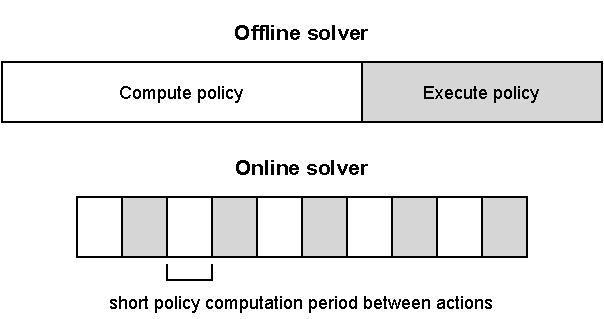
\includegraphics[width=0.6\textwidth]{figures/online-offline.pdf}
    \caption{Comparison of offline and online solving procedure}
\end{figure}

\noindent
There are two general approaches to solve POMDP: offline and online. Online solvers compute the optimal policy prior to execution for all possible future scenarios. Their advantage is that once the policy is found, policy execution is fast as there isonly a very minimal, negligible time overhead. However, offline planning is hard to scale to complex problems as the number of possible future scenarios grows exponentially with the size of the time horizon (curse of history). Furthermore, while the performance for small to medium sized POMDP can be quite good, computing the policy may take a very long time, and even small changes in the dynamics of the environment require a full recomputation \parencite{online_pomdp}. Online solvers interleave planning and plan execution. At every time step, only the current belief is considered to compute the next optimal action by searching ahead until a certain depth is reached. On the one hand, the scalability is greatly increased. On the other hand, sufficiently more online computation than with offline planning is required. The amount of available online planning time at each time step limits the performance. 

As discussed in Section \ref{sec:curses}, solving POMDP to optimality exactly is only feasible for small discrete POMDP. Larger POMDP are usually solved approximatelty. A wide range of offline and online approximate solvers is available. For discrete POMDP, most effective successful offline approximate solvers apply a form of \gls{pbvi}, where only a representative subset of the belief space is considered to approximate the value function \parencite{pomdp-point-based-value}. State-of the art methods include Perseus, and \gls{hsvi}. Perseus chooses belief states to consider by randomly sampling trajectories from an initial belief \parencite{pomdp_perseus}. It is sufficiently more compute efficient than PBVI but can suffer from a slow convergence behavior \parencite{pbvi-survey}. HSVI improves on Perseus potential slow convergence in large domains by constructing a belief search tree, maintaining the order in which beliefs are visited, in order to perform value updates in reverse order incrementally \parencite{solver_hsvi}.

Even the most advanced offline solvers reach their limit when dealing with large POMDP. Moreover, the state space of the POMDP for the shared control lane keeping task considered in this thesis has many continuous state variables (see Section \ref{sec:state}). Most offline solvers are not suited to be used with continuous states. There have been offline methods proposed to solve continuous POMDP, for example in \cite{pomdp-cont-offline}, and \cite{pomdp-cont-offline-2}. However, they have only been used for problems with relatively few state variables and are not considered further in this thesis. 

When it comes to online solvers, the paradigm of only trying to find a good local policy for the current belief state makes them sufficiently more efficient. The general approach is to construct a search tree rooted at the current belief, evaluating all possible further actions and observations. The methods differ in how the tree is explored to efficiently generate a good approximately optimal action to perform at the current belief. After this action has been performed in the real environment, the agent receives a reward and observation. On this basis, it updates its belief and the process repeats from the new belief. 

Recently, very promising results have been obtained for large POMDP using Monte Carlo sampling. Exploring the entire search tree is not feasible for deep time horizons because of the curse of history and the curse of dimensionality (see Section \ref{sec:curses}). \gls{mcts} methods address this issue by using a generative model to sample state transitions and observations (see Section \ref{sec:gen_model_intro}). By doing so, only a subset of histories is considered. The curse of dimensionality can be overcome in a similar fashion. Instead of evaluating all belief states, the start states for the search tree are sampled from the belief space. The number of belief states to consider can thereby be drastically reduced. 

% MCTS: The key idea is to evaluate each state in a search tree by the average outcome of simulations from that state.

% Another important issue for online POMDP planning is belief representation. Most online POMDP algorithms, including the Monte Carlo sampling algorithms, explicitly represent the belief as a probability distribution over the state space. This severely limits their scalability on POMDPs with very large state spaces, because a single belief update can take time quadratic in the number of states. Notable exceptions are POMCP and DESPOT. Both represent the belief as a set of sampled states and do not perform belief update over the entire state space during the online search.

\subsection{Online POMDP solving using Monte Carlo tree search}

The approach of using Monte Carlo sampling for both the choice of evaluated histories and estimating the belief was first applied in the \Glsentryfull{pomcp} algorithm by \cite{pomcp}. POMCP constructs a search tree of sampled histories. Each node stores its estimated value and sampled states that it corresponds to. The estimate is given by the return gained from forward simulations using the generative model during which the node is visited. The exploration is controlled using the \gls{ucb1} \parencite{ucb1} algorithm for action selection. The key idea is to aproximate the belief space using the same set of states that have been encountered during the forward search. Instead of representing the belief as a probability distribution over the states, it is given by the collection of states at the nodes. The underlying assumption is that if a state is more likely, it will be visited more often during the sampled trajectories. The relative number of times a state occurs in the collection defines its probability. Using this belief representation alleviates POMCP from expensive belief update calculations. POMCP has successfully been applied to approximately solve large POMDP. It is the solver used in this thesis. A detailed definition follows in Section \ref{sec:pomcp}. 

The \gls{despot} algorithm by \cite{despot} is a similar approach that can be seen as an evolution of POMCP. DESPOT is efficient as only a fixed number of sampled scenarios are considered. A scenario is a determinized trajectory in the belief tree that is defined in advance. At every depth of the belief tree, all actions but only a subset of resulting observations are considered. Thereby, the observation space is simplified. DESPOT's main advantage over POMCP is the ability to overcome POMCP's relatively poor worst-case behavior \parencite{pomcp-worst-case} caused by the UCB1 algorithm's tendency to overfit. DESPOT circumvents this by using regularization in the value function. Moreover, DESPOT is an anytime algorithm, building its tree incrementally. In addition to its value, at every node upper and lower bounds for its performance are maintained. First, a suboptimal policy is searched using heuristic search \parencite{solver_hsvi} and then it is incrementally improved upon. Branch-and-bound pruning is performed by pruning action nodes from the tree if their expected value is lower than the lower bound of another action. There are further extensions of DESPOT: HyPDESPOT is a parallelized version of DESPOT with significant performance enhancements \parencite{hyp-despot}. DESPOT-$\alpha$ further improves DESPOT's capability to handle very large observation and state spaces \parencite{despot-a}. And DESPOT-IS applies importance sampling to account for very rare events that are hard to sample \parencite{despot-is}. Unfortunately, DESPOT and its derivatives require the observation probability $Z$ to be explicitly known. This is not feasible for the shared control lane keeping task considered in this thesis.

\subsection{Solving continuous POMDP}

A continuous POMDP has continuous state, observation, and action spaces. This is the case for the scenario of lane keeping with a human in the loop that is examined in this thesis (see Section \ref{sec:lane_keeping_loop}). Hence, a solver that can handle continuous POMDP is required.

The aforementioned algorithms POMCP and DESPOT can natively be applied for continuous state spaces \parencite{pomcp_continuous}. As both use a collection of sampled states as their belief representation, they do not have to be adjusted to be able to represent beliefs about continuous states. These can also just be added to the collection if they occur during sample trajectories. It is unlikely that two identical continuous states are inserted. Therefore, the individual count of a state in the belief is rendered meaningless. Nevertheless, if the agent samples multiple similar situations, the corresponding states are also similar. For the continuous case, the assumed probability of being in a certain state is be given by the number of belief states that are close to it.

However, for continuous action and observation spaces the MCTS search tree used in POMCP and DESPOT degenerates. Only a single layer of nodes can be realized as every search leads to a new branch \parencite{online_pomdp_cont}. It is possible to discretize the action and observation spaces to bypass this limitation \parencite{pomcp_continuous}. Thereby, the continuous spaces are transformed into a discrete representation and the traditional methods are applicable. Action and observation discretization is performed in this thesis to be able to use POMCP. The details are discussed in Section \ref{sec:discretization}.

Solvers that work with fully continuous POMDP without discretization have been developed. POMCPOW is an extension of POMCP using progressive widening \parencite{online_pomdp_cont}. It uses weighted belief updates
and limits the amount of observations considered during planning. Observations are only gradually added to the lookahead tree as planning progresses. \gls{labecop} is another recent approach \parencite{online-cont-pomdp-2}. It is based on MCTS as well but avoids limiting the number of considered observations. As promising as these methods are, they again require the observation probabilities $Z$ to be known explicitly and are therefore not applicable to the problem addressed in this thesis.


% LABECOP incrementally samples a set
% of episodes H (b) , i.e. sequences of state-action-observation-
% reward quadruples starting from the current belief b ∈ B to
% compute an approximation of the optimal policy for b.
% Key to LABECOP is the realisation that the episodes in
% H (b) provide sufficient information to encode many different
% sequences of beliefs starting from b and that these beliefs,
% along with their approximated action values and corre-
% sponding action-selection strategy, can be extracted from
% H (b) on-the-fly during planning, without having to maintain
% a lookahead-tree.


% Approximate Solutions to POMDPs
% See (POMDP, Continuous, POMCPOW, POMCP-DOW, DPW, Thesis) SAFETY AND EFFICIENCY IN AUTONOMOUS VEHICLES THROUGH PLANNING WITH UNCERTAINTY


% Solving continuous POMDPs:
% See Towards Human-Like Prediction and Decision-Making for Automated Vehicles in Highway Scenarios

% See Monte Carlo Tree Search in (POMDP, Continuous, POMCPOW, POMCP-DOW, DPW, Thesis) SAFETY AND EFFICIENCY IN AUTONOMOUS VEHICLES THROUGH PLANNING WITH UNCERTAINTY

% Instead of using parametric forms, beliefs in continuous POMDPs can be represented with sets of particles (Thrun, 1999; Bai et al., 2011). Thrun proposes to use a particle filter for the belief updates and fitted value iteration for solving the POMDP. The proposed function approximator is K-nearest neighbors with the Kullback-Leibler divergence between kernel- based belief density estimates as distance metric. The repeated distance computations, which are expensive in high-dimensional spaces, represent a computational burden for this approach. Additionally, tuning is required for the parameters of the kernels. To escape these issues, Bai et al. combine a particle-based belief representation with the use of α-functions encoded as policy graphs to represent the value function (Bai et al., 2011). Instead of using policy graphs, which pose some limitations for long planning horizons, Brechtel et al. propose to represent the α-functions using regression trees (Brechtel et al., 2013; Brechtel, 2015). Finally, Sunberg and Kochenderfer propose an extension of POMCP that can handle fully continuous POMDPs by applying progressive widening to the action and observation spaces (Sunberg and Kochenderfer, 2018).